\documentclass{article}

\usepackage[utf8]{inputenc}
\usepackage[T1]{fontenc}
\usepackage[french]{babel}
\usepackage{graphicx}
\usepackage{hyperref}
\usepackage{caption}

\newcommand{\source}[1]{\caption*{Source: #1}}

\title{Optimisation de l'évacuation en cas d'urgence}

\begin{document}

\maketitle

\section{Étude des foules et évacuation}

L'étude du comportement des foules est un domaine important pour
améliorer la sécurité lors des évènement publics ainsi que dans
les bâtiments publics. Mais l'étude de ces foules par l'expérience
coute chère car il est nécessaire de mobiliser un grand nombre d'individus,
lors d'un simple festival de musique il peut y avoir plus de 7000 personnes.
De plus les personnes prenant pars aux expériences ne seront pas
dans les conditions réelles, ils ne seront pas paniqués par exemple,
l'expérience peut alors produire des résultats erronés.

La conception de bonnes expérience permettant l'étude des foules
étant difficile, l'étude se fait principalement grâce
à des simulations se basant sur des vidéo et des descriptions
d'évènements réelle ainsi que de résultats d'expériences.

\section{Objectifs}

L'objectif du TIPE de mon trinôme fut de développer ne programme
permettant d'étudier le mouvement d'une foule en cas d'évacuation
dans différentes situation. Puis d'en déduire des optimisations possibles
pour l'évacuation, particulièrement des optimisations concernant le plan
d'évacuation et la disposition des obstacles.

Le TIPE s'est découpé en deux simulations à des échelles différentes ainsi
qu'à une étude des résultats produit par les simulations, une des simulations
se base sur un graphe à flux variant et 
est à l'échelle d'un bâtiment, l'autre simulation se base sur les simulations
multi-agents et est à l'échelle d'une salle.

Je me suis concentré sur la modélisation du mouvement des agents dans la
simulation multi-agents.

\section{Simulation multi-agents}

Dans le domaine de la modélisation des foules les simulation multi-agents sont
les simulations les plus présentes. Contrairement aux modélisation se basant sur
des automates cellulaire et celles se basant sur le mouvement de particule
qui modélise le mouvement de la foule dans son ensemble, les modélisations
multi-agents modélise chaque agents individuellement le comportement de la foule
étant un résultat du comportement de chacun de ces agents.

\section{Outils utilisés}

Nous avons codé les simulations en Python car c'est le seule langage connue
par l'ensemble de notre trinôme, de plus Python viens avec un grand nombre
de modules permettant de faciliter le développement de notre simulation.

Nous avons utilisé un module de la librairie standard pour manipulé des
fichiers en JSON que nous avons utilisé comme
fichiers de configurations pour nos simulations permettant ainsi de facilité
l'étude de différentes situations.

Nous avons aussi utilisé le moteur physique en deux dimensions Pymunk,
qui est une enveloppe autour du moteur physique Chipmunk codé en C, pour
éviter de passer trop de notre temps voire tout notre temps sur la
modélisation physique des obstacles et des agents. Nous avons utilisé en
plus de Pymunk la librairie graphique Pygame pour afficher la simulation.

La structure de donnée utiliser par Pymunk pour ses calculs est une
hiérarchie de volumes englobants, une structure couramment utilisé pour la
détection de collisions dans un espace, c'est un arbre binaire dont chaque
nœuds est un volume qui englobe les volumes des nœuds enfants, les feuilles
de cette arbre sont les objets de l'espace \autoref{fig:BVH}. Ainsi pour chercher les
objets intersectant un objet donnée il suffit de rechercher récursivement
dans les sous arbres dont le volume englobant racine intersecte l'objet
donnée. Pymunk utilise des rectangles aligné aux axes des abscisses et des
ordonnées couramment nommé AABB -- axis-aligned bounding box -- comme
volume englobant.
Pour avoir des recherches efficaces Pymunk équilibre l'arbre en
minimisant la surface occupé par chaque nœuds.

\begin{figure}[h]
  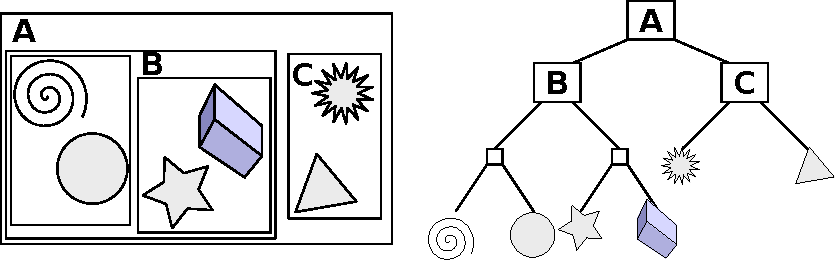
\includegraphics[height=4cm]{img/BVH.pdf}
  \caption{Un exemple de BVH}
  \source{\url{https://en.wikipedia.org/wiki/Bounding_volume_hierarchy}}
  \label{fig:BVH}
\end{figure}

\section{Description d'une salle}

Les salles dans lesquelles sont étudiées le mouvement sont délimité par
une AABB représentant les murs. Des trous dans les murs représentent les
différentes sorties. \autoref{fig:murs}

\begin{figure}[h]
  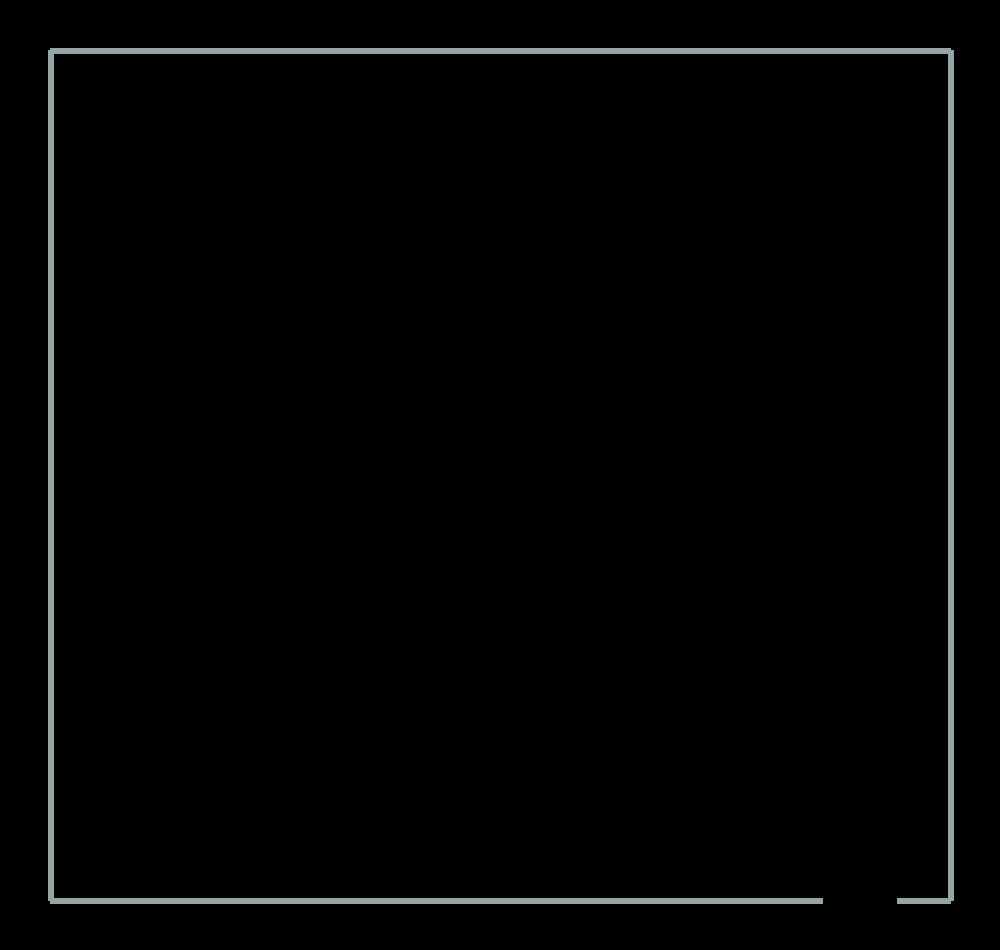
\includegraphics[height=4cm]{img/salle.png}
  \caption{Un exemple de salle, cette salle a une sortie en bas à droite}
  \label{fig:murs}
\end{figure}

Les obstacles présent dans la salles -- rangs d'une classe, pilier, etc... --
ont d'abord était représentés par des AABB \autoref{fig:obstacles} car ce
sont des formes très simples
et donc ont permis de rapidement développer une modélisation correcte. Puis
ces obstacles ont était représentés par des polygones convexes quelconques
\autoref{fig:obstacles} pour atteindre une modélisation plus générale, la convexité
ne pose pas
de problèmes dans la généralité car tout polygones peut se décomposer en une
union de polygones convexes -- il existe une triangulation pour tout
polygones simples -- on peut donc représenté tout obstacle en accolant des
polygones convexes ensembles mais ce n'est en générale pas nécessaire.

\begin{figure}[h]
  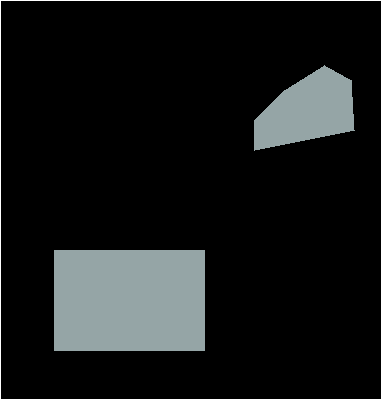
\includegraphics[height=4cm]{img/obstacles.png}
  \caption{Des exemples d'obstacles, une AABB à gauche et une polygone
    convexe quelconque à droite}
  \label{fig:obstacles}
\end{figure}

%Regarder une démonstration de la triangulation

\section{Description des agents}

Beaucoup de simplifications ont été faites pour les agents. Au mieux les agents
devrait être représentés par des ellipses souples car en vus de dessus les agents
ont grossièrement la forme d'ellipse et peuvent prendre plus ou moins de place
selon la pression qui leurs est appliqué -- ils plient les bras pour laisser de
la place par exemple --. Mais une ellipse est une forme qui engendre des calculs
de géométrie compliqué et lent à exécuté d'autant plus si l'ellipse est souple.
Nous avons donc choisis de représenter les agents par des disques rigides \autoref{fig:agent},
cela permet d'avoir une simulation rapide sans perdre trop de réalisme, les
disques étant une assez bonne approximation d'une ellipse et la différence
de rayons entre les cas extrêmes et petite par rapport au rayon moyen.

\begin{figure}[h]
  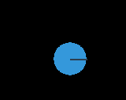
\includegraphics[height=4cm]{img/agent.png}
  \caption{Un agent}
  \label{fig:agent}
\end{figure}

%Essaye de trouver le rayon moyen et différence entre bras au repos et bras
%pressé contre soit

\section{Modélisation du mouvement d'un agent}

En situation réelle les agents ne prenant pas en compte ce qui se trouve
loin d'eux et ce qui
ne se trouve pas dans leurs champs de vision, ainsi 

\end{document}
